\documentclass[11pt,a4paper]{article}
\usepackage[utf8]{inputenc}
\usepackage{amsmath}
\usepackage{graphicx}
\usepackage{physics}

\usepackage{listings} 
\usepackage{xcolor}

\definecolor{codegreen}{rgb}{0,0.6,0}
\definecolor{codegray}{rgb}{0.5,0.5,0.5}
\definecolor{codepurple}{rgb}{0.58,0,0.82}
\definecolor{backcolour}{rgb}{0.95,0.95,0.92}

\lstdefinestyle{mystyle}{
    backgroundcolor=\color{backcolour},
    commentstyle=\color{codegreen},
    keywordstyle=\color{magenta},
    numberstyle=\tiny\color{codegray},
    stringstyle=\color{codepurple},
    basicstyle=\ttfamily\footnotesize,
    breakatwhitespace=false,
    breaklines=true,
    captionpos=b,
    keepspaces=true,
    numbers=left,
    numbersep=5pt,
    showspaces=false,
    showstringspaces=false,
    showtabs=false,
    tabsize=2
}

\lstset{style=mystyle}

\title{Computational Physics -- Problem Set 2}
\author{Tony Liu B05202068}

\begin{document}    
\maketitle

\section{Numerical Integration with Trapezoidal, Simpson, and 5-point formulas}%
\label{sec:numerical_integration_with_trapezoidal_simpson_and_5_point_formulas}

\begin{itemize}
    \item Trapezoidal rule\\
        $$ \int  _{x_0}^{x_1}dx f(x) = \frac{h}{2}\bigg(f(x_0) + f(x_1)\bigg) - \frac{1}{12}h^{3}f^{\prime \prime}(\xi)$$
    \item Simpson's rule\\
        $$  \int_{x_0}^{x_2}dx f(x) = \frac{h}{3}\bigg(f(x_0) + 4f(x_1) + f(x_2)\bigg) -\frac{1}{90}h^{5}f^{(4)}(\xi)$$

    \item Boole's rule(5-point formulas)\\
        $$  \int_{x_0}^{x_4}dx f(x) = \frac{2h}{45}\bigg(7f(x_0) + 32f(x_1) + 12f(x_2) + 32f(x_3) + 7f(x_4)\bigg) -\frac{8}{945}h^{7}f^{(6)}(\xi)$$

\end{itemize}
The above formulas can be derived from the Lagrange interpolating formula including the error term,
 \[
     f(x)\approx P_{n}(x) \equiv \sum _{i = 0}^{n}f(x_i)L_{i}(x)+\frac{f^{n+1}(\xi)}{(n+1)!}\prod_{i=0}^{n}(x-x_i)
,\]
where $$L_{i}(x) = \prod_{j \neq i}\frac{x-x_j}{x_i-x_j}.$$

Another more accurate method is based on Taylor expansion around the middle point (if the number of point is odd) with error term up to the next order. For example, for the Boole's rule, one takes the five points $x_0, x_1, x_2, x_3, x_4$ and makes the expansion around $x_2$:

\begin{multline*}
     f(x) = f(x_2) + f^{\prime}(x_2)(x-x_2)+\frac{f^{\prime \prime}(x_2)}{2!}(x-x_2)^{2} + \frac{f^{(3)}(x_2)}{3!}(x-x_2)^{3}\\
    + \frac{f^{(4)}(x_2)}{4!}(x-x_2)^{4} + \frac{f^{(5)}(x_2)}{5!}(x-x_2)^{5} + \frac{f^{(6)}(\xi)}{6!}(x-x_2)^{6}.
\end{multline*}

The integration from $x_0$ to  $x_4$ gives:
\begin{multline*}
    \int _{x_0} ^{x_4}dx f(x) =\int _{x_0} ^{x_4}dxf(x_2) +f^{\prime}(x_2) \int _{x_0} ^{x_4}dx(x-x_2)  + \frac{f^{\prime \prime}(x_2)}{2!}\int _{x_0} ^{x_4}dx(x-x_2)^{2} \\+ \frac{f^{(3)}(x_2)}{3!}\int _{x_0} ^{x_4}dx (x-x_2)^{3} +  \frac{f^{(4)}(x_2)}{4!}\int _{x_0} ^{x_4}dx (x-x_2)^{4} \\ + \frac{f^{(5)}(x_2)}{5!}\int _{x_0} ^{x_4}dx(x-x_2)^{5} +  \frac{f^{(6)}(\xi)}{6!}\int _{x_0} ^{x_4}dx(x-x_2)^{6}.$
\end{multline*}
\[
    \int _{x_0}^{x_4}dxf(x) = 4hf(x_2) +\frac{1}{3}(2h)^{3}f^{\prime \prime}(x_2) + \frac{2}{5}(2h)^{5}\frac{f^{(4)}(x_2)}{4!} + \frac{2}{7}(2h)^{7}\frac{f^{(6)}(\xi)}{6!}
.\]

From the 3-point formula for the second derivative of a function,

\begin{align*}   
f^{\prime \prime}(x_2) &= \frac{f(x_3) -2f(x_2) +f(x_1)}{h^2} - \frac{h^2}{12}f^{(4)}(x_2) -\frac{h^4}{360}f^{(6)}(\xi) \\
f^{\prime \prime}(x_2) &= \frac{f(x_3) -2f(x_2) +f(x_1)}{(2h)^2} - \frac{(2h)^2}{12}f^{(4)}(x_2) -\frac{(2h)^4}{360}f^{(6)}(\xi)
\end{align}
one can obtain $f^{\prime \prime}(x_2)$ to the forth order,
\[
    f^{\prime \prime}(x_2) = \frac{-f(x_4)+16f(x_3)-30f(x_2)+16f(x_1)- f(x_0)}{12h^2}+\frac{h^4}{30}f^{(6)}(\xi)    
,\]
and \[
    f^{(4)}(x_2) = \frac{f(x_4)-4f(x_3)+6f(x_2)-4f(x_1)+f(x_0)}{h^4} - \frac{h^2}{6}f^{(6)}(\xi)
.\]
Plug them to the integral with 5 points, one obtains the Boole's rule.

In the first problem, we would like to evaluate $$\int _{0}^{\pi}dx sin(x).$$ 
To do this, one uses the above approximation rule several times(assume $N$ is the mutiple of 4).
\newpage
\begin{itemize}
    \item   Extended trapezoidal rule
        $$\int _{x_0}^{x_N}dx f(x) = \Bigg( \int _{x_0}^{x_1} + \int _{x_1}^{x_2} + ... +\int _{x_{N-1}}^{x_N}\Bigg)dx f(x) $$
        $$= h\bigg( \frac{1}{2}f_0+f_1+...+f_{N-1} \frac{1}{2}f_N \bigg)-\frac{1}{12}Nh^3f^{\prime \prime}(\xi)$$


    \item Extended Simpson's rule
        $$\int _{x_0}^{x_N}dx f(x) = \Bigg( \int _{x_0}^{x_2} + \int _{x_2}^{x_4} + ... +\int _{x_{N-2}}^{x_N}\Bigg)dx f(x) $$
        $$= \frac{1}{3}h\bigg( f_0+4f_1+2f_2+...+4f_{N-1} +f_N \bigg)-\frac{1}{90}\frac{N}{2}h^5f^{\prime \prime}(\xi)$$
    \item Extended Boole's rule
$$\int _{x_0}^{x_N}dx f(x) = \Bigg( \int _{x_0}^{x_4} + \int _{x_4}^{x_8} + ... +\int _{x_{N-4}}^{x_N}\Bigg)dx f(x) $$
        $$= \frac{2}{45}h\bigg( 7f_0+32f_1+12f_2+32f_3+14f_4+...+32f_{N-1} +7f_N \bigg)-\frac{8}{945}\frac{N}{4}h^7f^{\prime \prime}(\xi)$$

\end{itemize}

Below is the table of the deviation of different rules from the exact value of the integral, which is $2$. In general, as expected, the 5-point formula gives the better approximation of the integral, since the error term of Boole's rule is up to $h^7$.

\begin{center}

\begin{tabular}{c c c c}

 N& Trapezoidal  & Simpson  & Boole \\
 4&	0.1038811207&		0.0045599937&		0.0014292002\\
 8&	0.0257682800&		0.0002691746&		0.0000169277\\
16&	0.0064297915&		0.0000166893&		0.0000004768\\
32&	0.0016074181&		0.0000004768&		0.0000004768\\
64&	0.0004006624&		0.0000007153&		0.0000007153\\
128&	0.0001002550&		0.0000001192&		0.0000001192\\
256&	0.0000286102&		0.0000035763&		0.0000036955\\
512&	0.0000121593&		0.0000042915&		0.0000051260\\
1024&	0.0000063181&		0.0000051260&		0.0000042915\\
\end{tabular}

\end{center}

\newpage
\section{Romberg Integration}%
\label{sec:romberg_integration}

For Romberg  integration, start with the trapezoidal rule:
$$T_{m,0} = h \Big(  \frac{f_0}{2} + f_1+ ...+f_{N-1}+\frac{f_N}{2}\Big).$$
Then according to the iteration formula:
$$T_{m+k,k}= \frac{4^kT_{m+k,k-1} - T_{m+k-1,k-1}}{4^k - 1},$$
one can write the code below to perform the iteration for the integral.
On the line $17$ to  $21$, I want to check whether the Romberg integration works according to:
 $$R_{m} = \frac{T_{m-1,0}-T_{m,0}}{T_{m,0} - T_{m+1,0}} \approx 4$$


\lstinputlisting[language=C, firstline=89, lastline=113]{Romberg_intg.c}


In the second problem, the integral we would like to evaluate is 
$$C(\nu) = \int _{0}^{\nu}d w cos\bigg(\frac{\pi w^2}{2}\bigg),  S(\nu) = \int _{0}^{\nu}d w sin\bigg(\frac{\pi w^2}{2}\bigg)$$
Here, I plot $$\frac{I}{I_0} = \frac{1}{2}\Bigg( (C(\nu)+0.5)^2 + (S(\nu)+0.5)^2 \Bigg)$$ as the function of $\nu$, ranging from $0$ to  $10$.

\begin{figure}
    \centering
    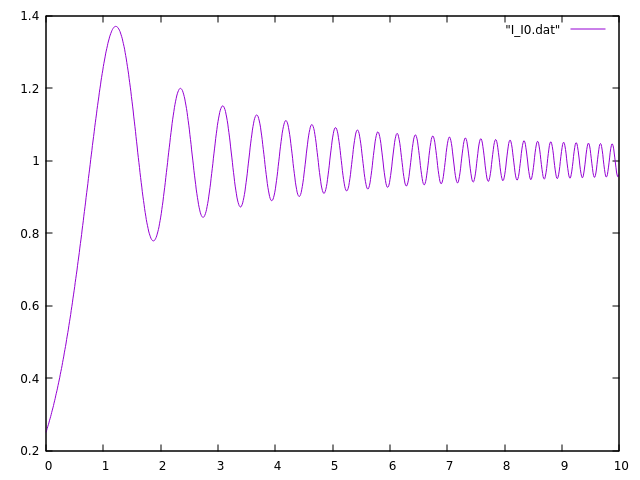
\includegraphics[width=0.9\linewidth]{I_I_0.png}
\end{figure}\\

The Romberg check at $\nu = 4.77 - 4.82$ is:\\

\begin{tabular}{c c c c c c c}
     $m$ / \nu&  4.77& 4.78& 4.79& 4.80& 4.81& 4.82\\
     2& 4.338214&   4.466623&   4.602847&   4.077215&   4.272999&   4.316915\\
     3& 4.083204&   4.240892&   4.114053&   3.593963&   3.908495&   4.157397\\
     4& 3.995094&   4.185833&   18.185184&  2.060869&   3.073088&   4.039226\\

\end{tabular}
As expected, the  $R_m$ is roughly equal to  $4,$ except for some irregular points.


\end{document}
   
   
